\documentclass{a0poster}
\usepackage{fancytikzposter} 
 
\usepackage[T1]{fontenc} 
\usepackage[cp1251]{inputenc}
\usepackage[russian]{babel}
\usepackage{graphicx}
\usepackage{graphics}
\usepackage{amssymb}
\usepackage{mathtext}
\usepackage{caption}
\usepackage{subcaption}
\usepackage{setspace}
\usepackage{amsmath}
\usepackage{amsthm}
\usepackage{lscape}
\usepackage{makecell}
\usepackage{multirow}
\usepackage{ulem}
\usepackage{indentfirst}
\usepackage{enumerate}

\usepackage[margin=\margin cm, paperwidth=84.1cm, paperheight=118.9cm]{geometry}

%%%%% --------- Change here if you want ---------- %%%%%
%% margin for the geometry package, must be changed before using the geometry package
%% default value is 4cm
% \setmargin{4}

%% the space between the blocks
%% default value is 2cm
% \setblockspacing{2}

%% the height of the title stripe in block nodes, decrease it to save space
%% default value is 3cm
% \setblocktitleheight{3}

%% the number of columns in the poster, possible values 2,3
%% default value is 2
% \setcolumnnumber{3}

%% the space between two or more groups of authors from different institutions
%% used in \maketitle
% \setinstituteshift{10}

\usetemplate{2}

%% components of the templates
%% (the maximal possible numbers are mentioned as the parameters)
% \usecolortemplate{4}
% \usebackgroundtemplate{5}
% \usetitletemplate{2}
% \useblocknodetemplate{5}
% \useplainblocktemplate{4}
% \useinnerblocktemplate{2}


%% the height of the head drawing on top 
%% applicable to templates N3, 4 and 5
 \setheaddrawingheight{17.3}


%% change the basic colors
%\definecolor{myblue}{HTML}{008888} 
%\setfirstcolor{myblue}% default 116699
%\setsecondcolor{gray!80!}% default CCCCCC
%\setthirdcolor{red!80!black}% default 991111

%% change the more specific colors
\setbackgrounddarkcolor{colorone!70!black}
% \setbackgroundlightcolor{colorone!70!}
% \settitletextcolor{textcolor}
% \settitlefillcolor{white}
% \settitledrawcolor{colortwo}
% \setblocktextcolor{textcolor}
% \setblockfillcolor{white}
% \setblocktitletextcolor{colorone}
% \setblocktitlefillcolor{colortwo} %the color of the border
% \setplainblocktextcolor{textcolor}
\setplainblockfillcolor{colorone!10!}
% \setplainblocktitletextcolor{textcolor}
\setplainblocktitlefillcolor{colorone!60!}
% \setinnerblocktextcolor{textcolor}
% \setinnerblockfillcolor{white}
% \setinnerblocktitletextcolor{white}
% \setinnerblocktitlefillcolor{colorthree}

%% changing the fonts
%\usepackage{cmbright}

\renewcommand\normalsize{\fontsize{32}{39.8pt}\selectfont}

%% add your packages here
\usepackage{hyperref}

\title{ Stability loss of zero balance state of nonlinear boundary-value problem \\
with deviate in boundary condition }
\author{ \textit{ Leonid Ivanovsky } \\
\textit{ P.G. Demidov Yaroslavl State University }
}

\begin{document}

%%%%% ---------- the background picture ---------- %%%%%
%% to change it modify the macro \BackgroundPicture
\ClearShipoutPicture
\AddToShipoutPicture{\BackgroundPicture}

\noindent % to have the picture right in the center
\begin{tikzpicture}
  \initializesizeandshifts
  % \setxshift{15}
  % \setyshift{2}

  %% the title block, #1 - shift, the default value is (0,0), #2 - width, #3 - scale
  %% the alias of the title block is `title', so we can refer to its boundaries later
  \ifthenelse{\equal{\template}{1}}{ 
    \titleblock{47}{1}
  }{
    \titleblock{47}{1.5}
  }

  %% a logo can be added to the title block
  %% #1 - anchor relative to the title block, #2 - shift, #3 - width, #3 - file name
  % \ifthenelse{\equal{\template}{2}}{ 
  %   \addlogo[south west]{(2,0)}{6cm}{unibz_b.png}
  % }{
  %   \addlogo[south west]{(2,0)}{6cm}{unibz_w.png}
  % }

  %%%%%%%%%% ------------------------------------------ %%%%%%%%%%
  \blocknodew{37}{ Boundary-value problem } %
  {
	\begin{equation}
		\dot u = u'' + \gamma u - u^3,	
	\end{equation}
	\begin{equation}
		u'(0, t) \, = 0, \quad u'(1, t) \, = \alpha\,u(x_0, t),
	\end{equation}
	
	$$ t \geqslant 0, \quad x \in [0,1], \quad \alpha, \gamma \in \mathbb{R}, \quad x_0 \in [0, 1). $$
  }
  
  \blocknodew{37}{ Eigenvalue problem } %
  { 
  $$ u(x, t) = e^{\lambda t} \, v(x). $$
  \vspace{0.4cm}
  \begin{equation}
  	v'' + (\gamma - \lambda)v = 0,	
  \end{equation}
  \begin{equation}	
  	v'(0) \, = 0, \qquad v'(1) \, = \alpha\,v(x_0).
  \end{equation}
  \vspace{0.4cm}
  $$ v(x) = c \ch  \mu x, \quad c \in \mathbb{R}, \quad \mu = \sqrt{-\gamma + \lambda}. $$
  }
  
  \blocknodew{37}{ Critical values of $\alpha$ } %
  {
  \begin{itemize}
  \item { $ \lambda = 0: \; \mu = \sqrt{-\gamma}, $ 
  }
  $$ \alpha_u = \frac{ \sqrt{-\gamma} \, \sh \sqrt{-\gamma} }{ \ch \sqrt{-\gamma} x_0 }. $$
  \item { $ \lambda = \pm i \omega: \; \mu = \sqrt{-\gamma + i \omega}, $ 
  }
  $$ \alpha_c = \frac{ \sqrt{-\gamma + i \omega} \, \sh \sqrt{-\gamma + i \omega} }{ \ch \sqrt{-\gamma + i \omega} x_0 }. $$
  \end{itemize}	
  }
  
  \blocknodew{37}{ Modeling of linearized boundary value problem } %
  {
	\begin{equation}\label{ivanovsky-eq3} \dot{u}_j =  n^2(u_{j+1} - 2u_j + u_{j-1}) + \gamma u_j, \quad j = \overline{1, n}, 
	\end{equation}
	\begin{equation}	
		u_0 = u_1, \quad u_{n+1} = 	u_n + \frac{\alpha}{n} u_k, \qquad k \in [1, n].
	\end{equation}
  }
  
  \blocknodew{37}{ Divergent loss of zero balance state $(\lambda = 0)$ } %
  { 
    \noindent\makebox[\textwidth][c]{
    \begin{minipage}[h]{0.65\linewidth}
	\center{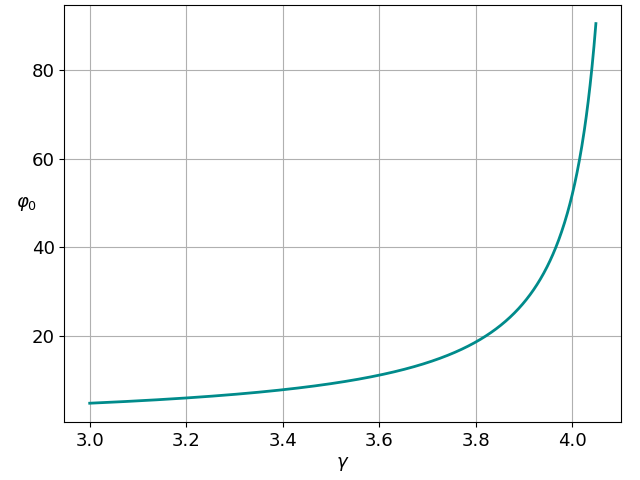
\includegraphics[width=0.65\linewidth]{divergent_phi0_0,00.png} }
	\end{minipage}
	}
	\hspace{0.5cm}
	\noindent\makebox[\textwidth][c]{
	\begin{minipage}[h]{0.65\linewidth}
	\center{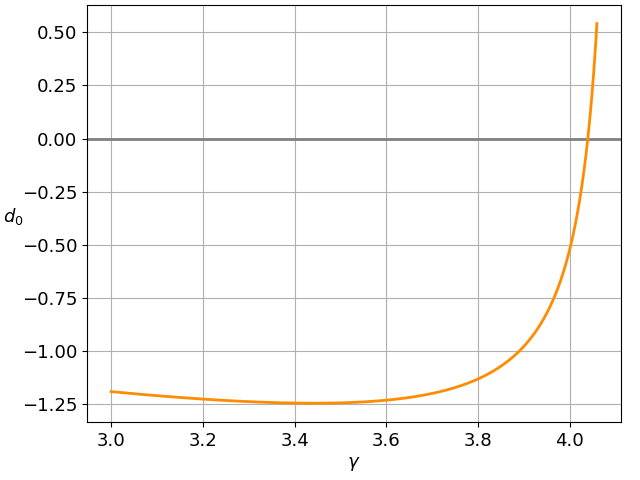
\includegraphics[width=0.65\linewidth]{divergent_d0_0,00.png} }
	\end{minipage}
	}
	$$ x_0 = 0.0 $$
  } 
  
  %%%%%%%%%%%%% NEW COLUMN %%%%%%%%%%%%%%% 
  \startsecondcolumn 

%%%%%%%%%% ------------------------------------------ %%%%%%%%%%
  
  \blocknodew{37}{ Normal form } %
  {
	\begin{equation}
	u = \sqrt{\varepsilon}u_0 + \varepsilon u_1 + \varepsilon^{\frac{3}{2}} u_2 + O(\varepsilon^2),\end{equation}
	
$$ \varepsilon = | \alpha - \alpha_{cr} |, $$
$$ \varepsilon \ll 1, \quad s = \varepsilon t. $$
  } 

  \blocknodew{37}{ Sequence of boundary value problems } %
  {
    \begin{equation}
		u_0 = u_0'' + \gamma u_0,
	\end{equation}
	\begin{equation}
		\dot u_2 + \frac{\partial u_0}{\partial s} = u_2'' + \gamma u_2 - u_0^3,
	\end{equation}
	\smallskip
	\begin{itemize}
	\item { $ \lambda = 0: \quad u_0 = z(s) \ch \mu x. $ }
	\item { $ \lambda = \pm i \omega: \quad u_0 = z(s) e^{i \omega t} \ch \mu x + \overline{z(s)} e^{-i \omega t} \overline{\ch \mu x}. $ }
	\end{itemize}
	
	\begin{equation}
		z' = \phi_0 z + d_0 z |z|^2.
	\end{equation}
  } 
   
  \blocknodew{37}{ Areas of stability for zero solution } %
  { 
    \noindent\makebox[\textwidth][c]{
    %\hspace{0.5cm}
	\begin{minipage}[h]{0.84\linewidth}
	\center{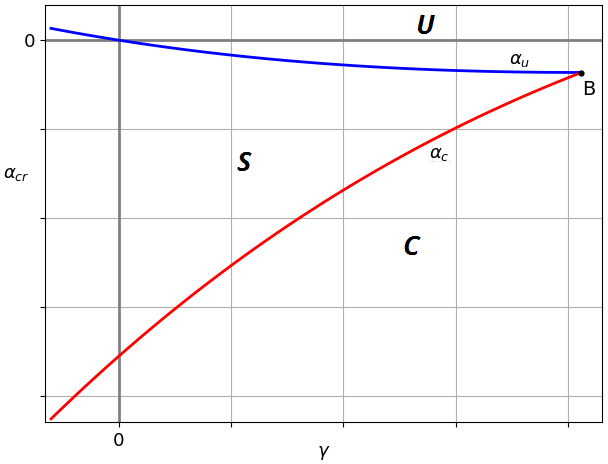
\includegraphics[width=0.84\linewidth]{scheme.png} }
	\end{minipage}
	}
\begin{minipage}{\linewidth}
        \coloredbox{colorthree!80!}{{\small This work was supported by the Russian Science Foundation (project \textnumero 18-29-10055).}}
     \end{minipage} 
  }  
  
  \blocknodew{37}{ Oscillating loss of zero balance state $(\lambda = \pm i \omega)$ } %
  { 
    \noindent\makebox[\textwidth][c]{
    \begin{minipage}[h]{0.65\linewidth}
	\center{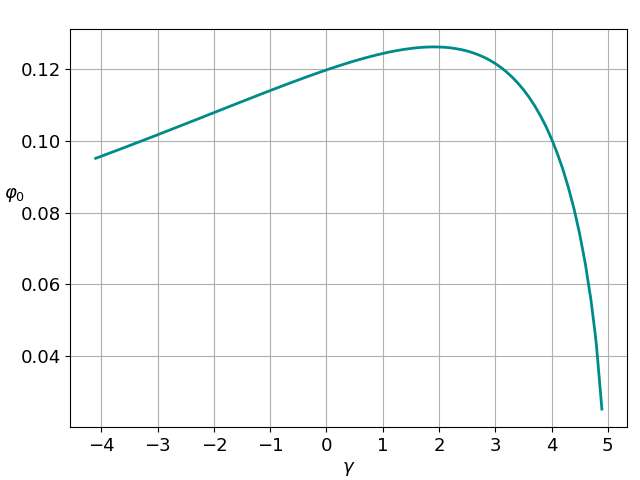
\includegraphics[width=0.65\linewidth]{oscillating_phi0_0,33.png} }
	\end{minipage}
	}	
	\hspace{0.5cm}
	\noindent\makebox[\textwidth][c]{
	\begin{minipage}[h]{0.65\linewidth}
	\center{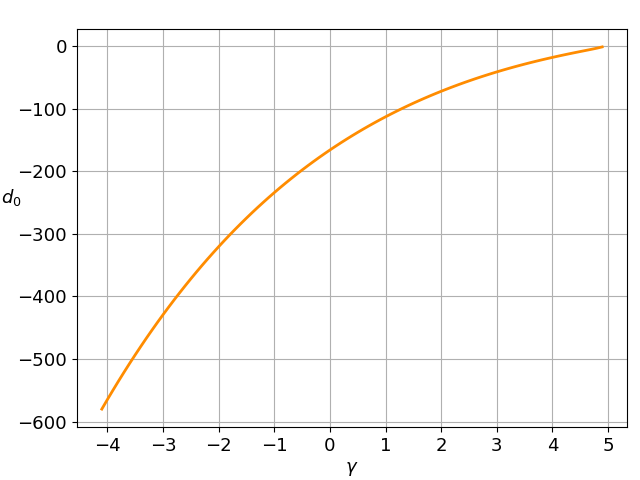
\includegraphics[width=0.65\linewidth]{oscillating_d0_0,33.png} }
	\end{minipage}
	}
	$$ x_0 = 0.33 $$
  } 

\end{tikzpicture}

\end{document}